% ===========================================================================
% Part I - Clustering (Experiments 1-4)
% ===========================================================================

\part{Clustering}

% ---------------------------------------------------------------------------
\chapter{Experiment 1: K-means Clustering}\label{exp:01}

\quickfacts
  {Dataset}{Mall Customers (\texttt{data/mall\_customers.csv}); 200 customers, 2 features (Annual Income, Spending Score)}
  {Key parameters}{K = 5, K-Means++ initialization, \texttt{n\_init} = 20, StandardScaler}
  {Headline result}{Silhouette 0.5547; Davies--Bouldin 0.5722; Calinski--Harabasz 248.65}

\section{Objective}
Partition unlabeled observations into $K$ clusters by iteratively assigning points to the
nearest centroid and updating centroids; choose $K$ with the elbow and silhouette diagnostics.

\section{Suggested Dataset}
Mall Customers (\texttt{data/mall\_customers.csv}), using Annual Income and Spending Score
as a two-dimensional, visualizable feature space. Features are standardized
(\texttt{StandardScaler}).

\section{Required Libraries}
numpy, pandas, matplotlib, scikit-learn.

\section{Brief Theory}
K-means minimizes the within-cluster sum of squared distances
\[
J = \sum_{k=1}^{K}\ \sum_{x_i \in C_k} \lVert x_i - \mu_k \rVert^2 ,
\]
by alternating two steps: assign every point to the nearest centroid, then set each
centroid to the mean of its assigned points. Each iteration never increases $J$, so the
algorithm converges --- but only to a \emph{local} optimum, which is why initialization
matters. \textbf{K-Means++} spreads the initial centroids by sampling them with probability
proportional to the squared distance to the nearest chosen centroid, giving lower and more
consistent inertia. Because Euclidean distance is scale-sensitive, numerical features should
be standardized. $K$ itself must be chosen externally: the \emph{elbow} (inertia) and the
\emph{silhouette} (cohesion vs.\ separation) are the standard diagnostics.

\section{Procedure}
\begin{enumerate}
  \item Load the dataset and retain the two numerical features.
  \item Standardize the features.
  \item Try $K = 2 \ldots 10$; record inertia (WCSS) and silhouette for each $K$.
  \item Choose $K$ at the elbow / silhouette peak and fit the final model with
        K-Means++ initialization, 20 restarts and a fixed random seed (see the code listing).
  \item Visualize the clusters and centroids.
  \item Report silhouette, Davies--Bouldin and Calinski--Harabasz.
\end{enumerate}

\section{Reference Implementation}
\begin{lstlisting}[style=mlcode,caption={Selecting K, then fitting the final K-means model}]
for k in range(2, 11):
    kmeans = KMeans(n_clusters=k, init='k-means++', n_init=10, random_state=42)
    kmeans.fit(X_mall_scaled)
    wcss.append(kmeans.inertia_)
    silhouette_scores.append(silhouette_score(X_mall_scaled, kmeans.labels_))

kmeans_model = KMeans(n_clusters=5, init='k-means++', n_init=20, random_state=42)
kmeans_labels = kmeans_model.fit_predict(X_mall_scaled)
\end{lstlisting}

\section{Evaluation / Expected Output}
Both the elbow curve and the silhouette curve indicate $K = 5$ (Figure~\ref{fig:exp01-elbow}).

\begin{figure}[htbp]
  \centering
  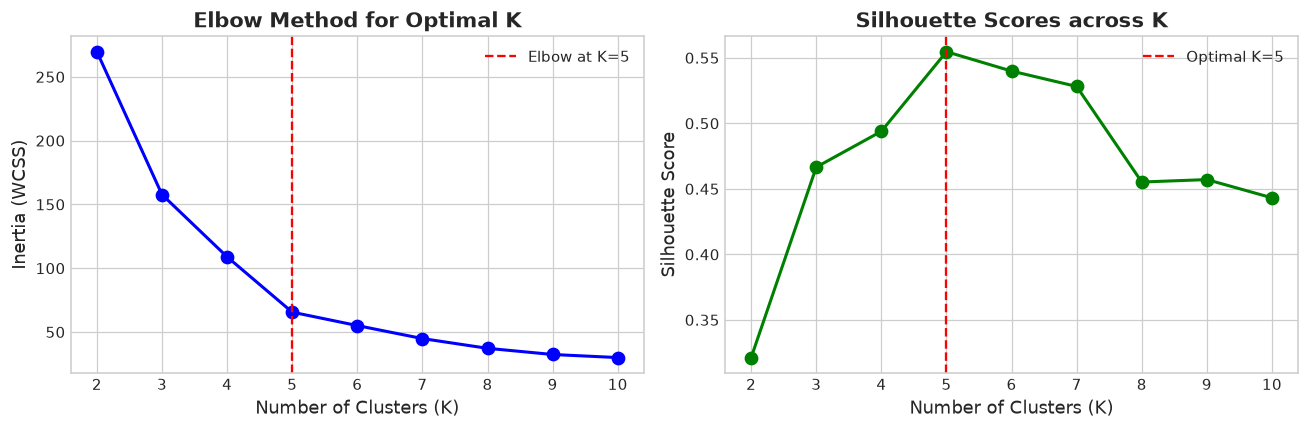
\includegraphics[width=0.95\textwidth]{figures/exp01_elbow_silhouette.png}
  \caption{Elbow (inertia) and silhouette curves for $K = 2 \ldots 10$; the elbow and the
  silhouette peak both occur at $K = 5$.}
  \label{fig:exp01-elbow}
\end{figure}

\begin{table}[htbp]
  \centering
  \caption{K-means evaluation on the standardized Mall Customers features.}
  \begin{tabular}{@{}lr@{}}
    \toprule
    \textbf{Metric} & \textbf{Value} \\
    \midrule
    Selected $K$ (elbow + silhouette peak) & 5 \\
    Silhouette score & \best{0.5547} \\
    Davies--Bouldin index & 0.5722 \\
    Calinski--Harabasz score & 248.65 \\
    \bottomrule
  \end{tabular}
\end{table}

Silhouette $\approx 0.55$ indicates compact, reasonably separated clusters on real data;
Davies--Bouldin $< 1$ confirms good separation.

\section{Viva / Discussion Questions}
\begin{description}
  \item[Why does K-means depend on feature scaling?] It minimizes Euclidean distance;
  unscaled features with larger ranges dominate the distance and therefore the assignments.
  \item[What is inertia?] The within-cluster sum of squared distances to the centroids
  (WCSS); lower is tighter, but it always decreases with $K$, so it is not a standalone
  quality score.
  \item[Why can a high silhouette score still be misleading?] It favors compact convex
  clusters and can be high for a trivial partition; it misjudges elongated or
  density-varying structures.
  \item[What happens when clusters are non-spherical?] K-means splits them with straight
  Voronoi boundaries and merges elongated clusters incorrectly (see Experiment 5).
  \item[Why is K-Means++ preferred over random initialization?] It spreads the initial
  centroids out, reducing convergence to poor local optima and giving more stable inertia.
\end{description}

\section{Complete Code Listing}
% ===========================================================================
% exp01_kmeans.tex - complete code listings for Experiment 1
% Source: notebooks/01_clustering_algorithms.ipynb (executed)
% ===========================================================================

\begin{codebox}[title={Listing 1.1 Imports and plotting style}]
# ---- Core numerical and plotting libraries ----
import os
import numpy as np
import pandas as pd
import matplotlib.pyplot as plt
import seaborn as sns


# ---- Scikit-Learn clustering models ----
from sklearn.cluster import KMeans, AgglomerativeClustering
# ---- Feature scaling + unsupervised evaluation metrics ----
from sklearn.preprocessing import StandardScaler
from sklearn.metrics import silhouette_score, davies_bouldin_score, calinski_harabasz_score
# ---- SciPy hierarchical clustering utilities (linkage + dendrogram) ----
from scipy.cluster.hierarchy import dendrogram, linkage

# Styling setup (consistent look across all notebooks)
plt.style.use('seaborn-v0_8-whitegrid' if 'seaborn-v0_8-whitegrid' in plt.style.available else 'default')
plt.rcParams['font.sans-serif'] = 'DejaVu Sans'
plt.rcParams['figure.figsize'] = (10, 6)
plt.rcParams['figure.dpi'] = 110

# Fix the random seed so every run reproduces the same results
np.random.seed(42)
print("Libraries successfully imported!")
\end{codebox}

\begin{codebox}[title={Listing 1.2 Load and preprocess the Mall Customers data}]
# ---- Load the Mall Customers dataset ----
df_mall = pd.read_csv('../data/mall_customers.csv')
print("Dataset Shape:", df_mall.shape)
print(df_mall.head(3))

# ---- Feature selection: two features so the clusters can be shown in 2D ----
X_mall = df_mall[['Annual Income (k$)', 'Spending Score (1-100)']].values

# ---- Standardize (mean = 0, std = 1): distance-based algorithms are scale-sensitive ----
scaler = StandardScaler()
X_mall_scaled = scaler.fit_transform(X_mall)
\end{codebox}

\begin{codebox}[title={Listing 1.3 Select K with the elbow and silhouette curves}]
# ---- Selecting the optimal number of clusters K ----
# Try K = 2..10 and record two diagnostics:
#   * Inertia (WCSS): total squared distance from points to their centroid
#   * Silhouette score: cluster cohesion vs. separation
k_range = range(2, 11)
wcss = []
silhouette_scores = []

for k in k_range:
    # n_init=10 runs K-Means from 10 different seeds and keeps the best run
    kmeans = KMeans(n_clusters=k, init='k-means++', n_init=10, random_state=42)
    kmeans.fit(X_mall_scaled)
    wcss.append(kmeans.inertia_)                                               # WCSS of the fitted model
    silhouette_scores.append(silhouette_score(X_mall_scaled, kmeans.labels_))  # partition quality

fig, (ax1, ax2) = plt.subplots(1, 2, figsize=(12, 4))

# ---- Left: elbow curve (look for the "knee" where inertia stops falling quickly) ----
ax1.plot(k_range, wcss, 'bo-', linewidth=2, markersize=8)
ax1.set_title("Elbow Method for Optimal K", fontsize=14, fontweight='bold')
ax1.set_xlabel("Number of Clusters (K)", fontsize=12)
ax1.set_ylabel("Inertia (WCSS)", fontsize=12)
ax1.axvline(x=5, color='r', linestyle='--', label='Elbow at K=5')
ax1.legend()

# ---- Right: silhouette score for each K (higher is better) ----
ax2.plot(k_range, silhouette_scores, 'go-', linewidth=2, markersize=8)
ax2.set_title("Silhouette Scores across K", fontsize=14, fontweight='bold')
ax2.set_xlabel("Number of Clusters (K)", fontsize=12)
ax2.set_ylabel("Silhouette Score", fontsize=12)
ax2.axvline(x=5, color='r', linestyle='--', label='Optimal K=5')
ax2.legend()

plt.tight_layout()
plt.show()
\end{codebox}

\begin{codebox}[title={Listing 1.4 Final K-means model (K = 5)}]
# ---- Final K-Means model with the selected K = 5 ----
optimal_k = 5
kmeans_model = KMeans(n_clusters=optimal_k, init='k-means++', n_init=20, random_state=42)
kmeans_labels = kmeans_model.fit_predict(X_mall_scaled)  # hard cluster assignment per sample

print(f"K-Means Silhouette Score: {silhouette_score(X_mall_scaled, kmeans_labels):.4f}")
print(f"K-Means Davies-Bouldin Index: {davies_bouldin_score(X_mall_scaled, kmeans_labels):.4f}")
\end{codebox}


% ---------------------------------------------------------------------------
\chapter{Experiment 2: Modified K-means}\label{exp:02}

\quickfacts
  {Dataset}{Mall Customers (200 $\times$ 2, standardized)}
  {Key parameters}{K-Means++ initialization; outlier threshold = 97th percentile of centroid distances}
  {Headline result}{Distance threshold 1.072; 6 of 200 observations flagged as candidate outliers}

\section{Objective}
Implement a transparent modification of K-means that uses K-Means++ initialization and an
explicit outlier-distance check before final cluster interpretation.

\section{Suggested Dataset}
Mall Customers (200 $\times$ 2, standardized). The modification is applied on top of the same
features.

\section{Required Libraries}
numpy, matplotlib, scikit-learn.

\section{Brief Theory}
There is no single universally accepted algorithm named ``modified K-means''; variants
differ by application. In this lab the modification is intentionally defined so that it can
be reproduced exactly:
\begin{enumerate}
  \item initialize the centroids with \textbf{K-Means++} (spread-out seeds);
  \item fit standard K-means and obtain the hard labels;
  \item compute each sample's distance to its \emph{assigned} centroid,
        $d_i = \lVert x_i - \mu_{c_i} \rVert$;
  \item set a threshold from a documented percentile of the training distances
        (97th percentile here);
  \item flag samples with $d_i$ beyond the threshold as \textbf{candidate outliers}.
\end{enumerate}
This is an experimental variant that adds outlier awareness to the standard algorithm; it
is not a standard replacement for robust clustering methods.

\section{Procedure}
\begin{enumerate}
  \item Fit K-means with K-Means++ initialization, $K = 5$.
  \item Compute $d_i = \lVert x_i - \mu_{c_i} \rVert$ for every sample.
  \item Set the threshold to the 97th percentile of the training distances.
  \item Flag samples with $d_i > \text{threshold}$ as candidate outliers.
  \item Plot the clusters with the flagged points highlighted.
  \item Compare the modified interpretation with the standard labels.
\end{enumerate}

\section{Reference Implementation}
\begin{lstlisting}[style=mlcode,caption={K-Means++ followed by the outlier-distance check}]
km_mod = KMeans(n_clusters=5, init='k-means++', n_init=20, random_state=42)
mod_labels = km_mod.fit_predict(X_mall_scaled)

dist_to_centroid = np.linalg.norm(X_mall_scaled - km_mod.cluster_centers_[mod_labels], axis=1)
threshold = np.percentile(dist_to_centroid, 97)
outlier_flag = dist_to_centroid > threshold
\end{lstlisting}

\section{Evaluation / Expected Output}
\begin{table}[htbp]
  \centering
  \caption{Modified K-means: outlier-distance check on the standardized features.}
  \begin{tabular}{@{}lr@{}}
    \toprule
    \textbf{Item} & \textbf{Value} \\
    \midrule
    Distance threshold (97th percentile) & 1.072 (standardized units) \\
    Flagged candidate outliers & \best{6 of 200 (3\%)} \\
    Cluster labels & identical to standard K-means \\
    Silhouette / Davies--Bouldin (same partition) & 0.5547 / 0.5722 \\
    \bottomrule
  \end{tabular}
\end{table}

The flagged customers are the most weakly attached points of their clusters --- typically
boundary customers with unusual income/spending combinations. The cluster structure itself
is unchanged, which is expected: the modification adds an outlier interpretation layer.

\section{Viva / Discussion Questions}
\begin{description}
  \item[Why is it important to define a modification precisely?] Without a formal definition
  ``modified K-means'' is ambiguous; fixing the initialization, the distance measure and the
  percentile rule makes the experiment reproducible and testable.
  \item[How does K-Means++ differ from random initialization?] K-Means++ selects initial
  centroids with probability proportional to the squared distance to the nearest chosen
  centroid, spreading the seeds out and avoiding poor local optima.
  \item[Why might distance-to-centroid fail for elongated clusters?] Centroid distance is
  isotropic; a point can be close to the centroid along the long axis yet far along the short
  axis, so elongated clusters can flag legitimate points and hide real outliers.
\end{description}

\section{Complete Code Listing}
% ===========================================================================
% exp02_modified_kmeans.tex - complete code listings for Experiment 2
% Source: notebooks/01_clustering_algorithms.ipynb (executed)
% ===========================================================================

\begin{lstlisting}[style=mlcode,caption={Core numerical and plotting libraries}]
# ---- Core numerical and plotting libraries ----
import os
import numpy as np
import pandas as pd
import matplotlib.pyplot as plt
import seaborn as sns


# ---- Scikit-Learn clustering models ----
from sklearn.cluster import KMeans, AgglomerativeClustering
# ---- Feature scaling + unsupervised evaluation metrics ----
from sklearn.preprocessing import StandardScaler
from sklearn.metrics import silhouette_score, davies_bouldin_score, calinski_harabasz_score
# ---- SciPy hierarchical clustering utilities (linkage + dendrogram) ----
from scipy.cluster.hierarchy import dendrogram, linkage

# Styling setup (consistent look across all notebooks)
plt.style.use('seaborn-v0_8-whitegrid' if 'seaborn-v0_8-whitegrid' in plt.style.available else 'default')
plt.rcParams['font.sans-serif'] = 'DejaVu Sans'
plt.rcParams['figure.figsize'] = (10, 6)
plt.rcParams['figure.dpi'] = 110

# Fix the random seed so every run reproduces the same results
np.random.seed(42)
print("Libraries successfully imported!")
\end{lstlisting}

\begin{lstlisting}[style=mlcode,caption={Load the Mall Customers dataset}]
# ---- Load the Mall Customers dataset ----
df_mall = pd.read_csv('../data/mall_customers.csv')
print("Dataset Shape:", df_mall.shape)
print(df_mall.head(3))

# ---- Feature selection: two features so the clusters can be shown in 2D ----
X_mall = df_mall[['Annual Income (k$)', 'Spending Score (1-100)']].values

# ---- Standardize (mean = 0, std = 1): distance-based algorithms are scale-sensitive ----
scaler = StandardScaler()
X_mall_scaled = scaler.fit_transform(X_mall)
\end{lstlisting}

\begin{lstlisting}[style=mlcode,caption={Modified K-Means (manual variant): K-Means++ + outlier-distance check}]
# ---- Modified K-Means (manual variant): K-Means++ + outlier-distance check ----
km_mod = KMeans(n_clusters=optimal_k, init='k-means++', n_init=20, random_state=42)
mod_labels = km_mod.fit_predict(X_mall_scaled)

# Distance of every sample to its assigned centroid
dist_to_centroid = np.linalg.norm(X_mall_scaled - km_mod.cluster_centers_[mod_labels], axis=1)
threshold = np.percentile(dist_to_centroid, 97)      # documented percentile
outlier_flag = dist_to_centroid > threshold

print(f"Distance threshold (97th percentile): {threshold:.3f}")
print(f"Flagged candidate outliers: {outlier_flag.sum()} of {len(X_mall)}")

# ---- Plot clusters with flagged candidate outliers highlighted ----
plt.figure(figsize=(9, 6))
for cluster_id in range(optimal_k):
    pts = X_mall[mod_labels == cluster_id]
    plt.scatter(pts[:, 0], pts[:, 1], s=45, edgecolors='k', alpha=0.8)
plt.scatter(X_mall[outlier_flag, 0], X_mall[outlier_flag, 1], s=180, facecolors='none',
            edgecolors='red', linewidths=2.5, label=f'Flagged outliers ({outlier_flag.sum()})')
plt.title("Modified K-Means: K-Means++ with Outlier-Distance Flagging", fontsize=13, fontweight='bold')
plt.xlabel("Annual Income (k$)", fontsize=12)
plt.ylabel("Spending Score (1-100)", fontsize=12)
plt.legend()
plt.tight_layout()
plt.show()
\end{lstlisting}


% ---------------------------------------------------------------------------
\chapter{Experiment 3: Hierarchical Clustering}\label{exp:03}

\quickfacts
  {Dataset}{Mall Customers (200 $\times$ 2, standardized)}
  {Key parameters}{Ward linkage; cut at $K = 5$; truncated dendrogram (last 25 merges)}
  {Headline result}{Silhouette 0.5538; Davies--Bouldin 0.5779; Calinski--Harabasz 244.41}

\section{Objective}
Perform agglomerative hierarchical clustering and interpret the resulting dendrogram and
cluster labels.

\section{Suggested Dataset}
Mall Customers (200 $\times$ 2, standardized).

\section{Required Libraries}
scipy, scikit-learn, matplotlib.

\section{Brief Theory}
Agglomerative clustering starts with one cluster per point and repeatedly merges the closest
pair of clusters. With \textbf{Ward linkage} the merge cost is the increase in total
within-cluster variance,
\[
\Delta W(A, B) = \frac{n_A n_B}{n_A + n_B}\,\lVert \mu_A - \mu_B \rVert^2 ,
\]
so the algorithm always merges the pair whose combination loses the least compactness. The
dendrogram records every merge and its height (distance); cutting it at a chosen height
yields a flat partition with the desired number of clusters.

\section{Procedure}
\begin{enumerate}
  \item Standardize the features.
  \item Compute the Ward linkage matrix.
  \item Plot the dendrogram (truncated for readability) and choose a cut level.
  \item Fit \texttt{AgglomerativeClustering} with $K = 5$ and Ward linkage.
  \item Evaluate with silhouette, Davies--Bouldin and Calinski--Harabasz.
  \item Discuss the choice of linkage.
\end{enumerate}

\section{Reference Implementation}
\begin{lstlisting}[style=mlcode,caption={Ward linkage, dendrogram and the final agglomerative model}]
linkage_matrix = linkage(X_mall_scaled, method='ward')
dendrogram(linkage_matrix, truncate_mode='lastp', p=25, show_contracted=True)

agg_model = AgglomerativeClustering(n_clusters=5, metric='euclidean', linkage='ward')
agg_labels = agg_model.fit_predict(X_mall_scaled)
\end{lstlisting}

\section{Evaluation / Expected Output}
The dendrogram (Figure~\ref{fig:exp03-dendro}) shows a clear large merge gap that supports
cutting at five clusters.

\begin{figure}[htbp]
  \centering
  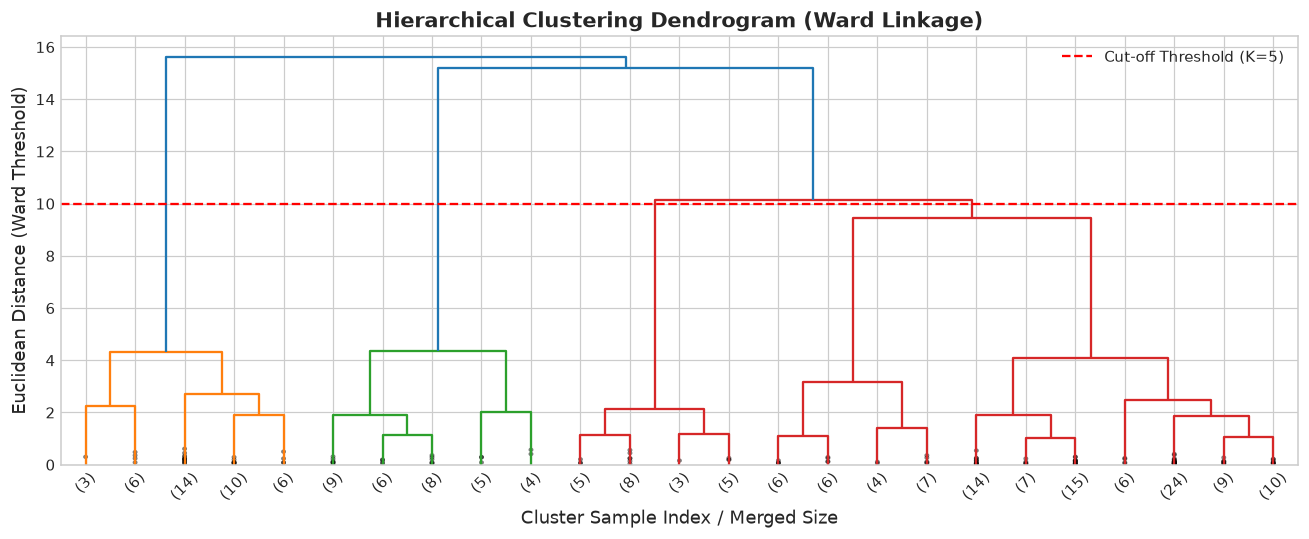
\includegraphics[width=0.92\textwidth]{figures/exp03_dendrogram.png}
  \caption{Hierarchical clustering dendrogram (Ward linkage, truncated to the last 25
  merges); the dashed line marks the cut that yields $K = 5$.}
  \label{fig:exp03-dendro}
\end{figure}

\begin{table}[htbp]
  \centering
  \caption{Hierarchical (Ward) clustering evaluation on the standardized features.}
  \begin{tabular}{@{}lr@{}}
    \toprule
    \textbf{Metric} & \textbf{Value} \\
    \midrule
    Silhouette score & 0.5538 \\
    Davies--Bouldin index & 0.5779 \\
    Calinski--Harabasz score & 244.41 \\
    \bottomrule
  \end{tabular}
\end{table}

The partition is nearly identical in quality to K-means (silhouette difference below 0.001),
but requires no initialization and exposes the full merge hierarchy.

\section{Viva / Discussion Questions}
\begin{description}
  \item[What does a dendrogram show?] The complete merge hierarchy: leaf order, merge heights
  (distances) and the nested cluster structure; cutting at a height produces a flat partition.
  \item[What is linkage?] The rule that defines the distance between two clusters:
  single (closest pair), complete (farthest pair), average (mean pair) or Ward (variance
  increase).
  \item[When is Ward linkage inappropriate?] With strongly non-spherical/elongated clusters,
  very unequal cluster sizes or heavy outliers --- it assumes compact clusters of similar
  variance.
\end{description}

\section{Complete Code Listing}
% ===========================================================================
% exp03_hierarchical.tex - complete code listings for Experiment 3
% Source: notebooks/01_clustering_algorithms.ipynb (executed)
% ===========================================================================

\begin{codebox}[title={Core numerical and plotting libraries}]
# ---- Core numerical and plotting libraries ----
import os
import numpy as np
import pandas as pd
import matplotlib.pyplot as plt
import seaborn as sns


# ---- Scikit-Learn clustering models ----
from sklearn.cluster import KMeans, AgglomerativeClustering
# ---- Feature scaling + unsupervised evaluation metrics ----
from sklearn.preprocessing import StandardScaler
from sklearn.metrics import silhouette_score, davies_bouldin_score, calinski_harabasz_score
# ---- SciPy hierarchical clustering utilities (linkage + dendrogram) ----
from scipy.cluster.hierarchy import dendrogram, linkage

# Styling setup (consistent look across all notebooks)
plt.style.use('seaborn-v0_8-whitegrid' if 'seaborn-v0_8-whitegrid' in plt.style.available else 'default')
plt.rcParams['font.sans-serif'] = 'DejaVu Sans'
plt.rcParams['figure.figsize'] = (10, 6)
plt.rcParams['figure.dpi'] = 110

# Fix the random seed so every run reproduces the same results
np.random.seed(42)
print("Libraries successfully imported!")
\end{codebox}

\begin{codebox}[title={Load the Mall Customers dataset}]
# ---- Load the Mall Customers dataset ----
df_mall = pd.read_csv('../data/mall_customers.csv')
print("Dataset Shape:", df_mall.shape)
print(df_mall.head(3))

# ---- Feature selection: two features so the clusters can be shown in 2D ----
X_mall = df_mall[['Annual Income (k$)', 'Spending Score (1-100)']].values

# ---- Standardize (mean = 0, std = 1): distance-based algorithms are scale-sensitive ----
scaler = StandardScaler()
X_mall_scaled = scaler.fit_transform(X_mall)
\end{codebox}

\begin{codebox}[title={Build the linkage matrix and draw the dendrogram}]
# ---- Build the linkage matrix and draw the dendrogram ----
# 'ward' linkage merges the pair of clusters that increases within-cluster variance the least.
linkage_matrix = linkage(X_mall_scaled, method='ward')

# The dendrogram shows every merge; we truncate it to the last 25 merges for readability.
plt.figure(figsize=(12, 5))
dendrogram(
    linkage_matrix,
    truncate_mode='lastp',   # show only the last p merged clusters
    p=25,
    leaf_rotation=45,
    leaf_font_size=10,
    show_contracted=True     # condensed leaves are shown as counts
)
plt.title("Hierarchical Clustering Dendrogram (Ward Linkage)", fontsize=14, fontweight='bold')
plt.xlabel("Cluster Sample Index / Merged Size", fontsize=12)
plt.ylabel("Euclidean Distance (Ward Threshold)", fontsize=12)
plt.axhline(y=10.0, color='r', linestyle='--', label='Cut-off Threshold (K=5)')  # horizontal cut => cluster count
plt.legend()
plt.tight_layout()
plt.show()
\end{codebox}

\begin{codebox}[title={Fit the final Agglomerative model (Ward linkage, K = 5)}]
# ---- Fit the final Agglomerative model (Ward linkage, K = 5) ----
agg_model = AgglomerativeClustering(n_clusters=optimal_k, metric='euclidean', linkage='ward')
agg_labels = agg_model.fit_predict(X_mall_scaled)

print(f"Hierarchical Silhouette Score: {silhouette_score(X_mall_scaled, agg_labels):.4f}")
print(f"Hierarchical Davies-Bouldin Index: {davies_bouldin_score(X_mall_scaled, agg_labels):.4f}")
\end{codebox}


% ---------------------------------------------------------------------------
\chapter{Experiment 4: Fuzzy C-means}\label{exp:04}

\quickfacts
  {Dataset}{Mall Customers (200 $\times$ 2, standardized); $K = 5$}
  {Key parameters}{Fuzzifier $m = 2.0$; tolerance $10^{-5}$; maximum 150 iterations}
  {Headline result}{Silhouette 0.5547; Fuzzy Partition Coefficient (FPC) 0.6711}

\section{Objective}
Cluster data using fuzzy memberships so that each observation can belong to multiple
clusters with different degrees of membership.

\section{Suggested Dataset}
Mall Customers (200 $\times$ 2, standardized), $K = 5$, fuzzifier $m = 2.0$.

\section{Required Libraries}
numpy, pandas, matplotlib (the c-means equations are implemented from scratch;
\texttt{scikit-fuzzy} is an equivalent library implementation).

\section{Brief Theory}
Unlike hard K-means, Fuzzy C-means assigns every sample $x_i$ a membership degree
$u_{ik} \in [0,1]$ in every cluster, with $\sum_{k=1}^{K} u_{ik} = 1$. It minimizes
\[
J_m = \sum_{i=1}^{N}\sum_{k=1}^{K} u_{ik}^{m}\,\lVert x_i - v_k \rVert^2 , \qquad m > 1 ,
\]
by alternating two updates until convergence:
\[
v_k = \frac{\sum_i u_{ik}^{m} x_i}{\sum_i u_{ik}^{m}},
\qquad
u_{ik} = \frac{1}{\sum_{j=1}^{K}\left(\frac{d_{ik}}{d_{ij}}\right)^{2/(m-1)}} .
\]
The fuzzifier $m$ controls how soft the memberships are ($m \to 1$ approaches K-means). The
\textbf{Fuzzy Partition Coefficient} $\mathrm{FPC} = \frac{1}{N}\sum_i \sum_k u_{ik}^2$
measures the fuzziness of the result ($1$ = completely hard, $1/K$ = maximally fuzzy).

\section{Procedure}
\begin{enumerate}
  \item Standardize the data.
  \item Initialize the membership matrix randomly, with each row summing to 1.
  \item Alternate the centroid and membership updates until $\max|\Delta U| < 10^{-5}$.
  \item Derive hard labels with $\arg\max_k u_{ik}$.
  \item Report the clustering metrics and the FPC; visualize the hard partition.
  \item Identify ambiguous samples with near-uniform membership vectors.
\end{enumerate}

\section{Reference Implementation}
\begin{lstlisting}[style=mlcode,caption={Core alternating updates of Fuzzy C-means}]
Um = U ** self.m
centers = np.dot(Um.T, X) / Um.sum(axis=0)[:, np.newaxis]
dist = np.linalg.norm(X[:, np.newaxis, :] - centers[np.newaxis, :, :], axis=2) + 1e-10
U = (1.0 / dist) ** (2.0 / (self.m - 1.0))
U = U / U.sum(axis=1, keepdims=True)
labels = np.argmax(U, axis=1)
\end{lstlisting}

\section{Evaluation / Expected Output}
\begin{table}[htbp]
  \centering
  \caption{Fuzzy C-means evaluation ($K = 5$, $m = 2.0$).}
  \begin{tabular}{@{}lr@{}}
    \toprule
    \textbf{Metric} & \textbf{Value} \\
    \midrule
    Silhouette score (hard labels) & 0.5547 \\
    Davies--Bouldin index & 0.5722 \\
    Fuzzy Partition Coefficient (FPC) & \best{0.6711} \\
    Iterations to convergence & fewer than 50 \\
    \bottomrule
  \end{tabular}
\end{table}

FPC $= 0.67$ (between $1/K = 0.2$ and $1.0$) shows that the partition is mostly crisp but
retains soft boundary memberships. Figure~\ref{fig:exp01-grid} compares the four clustering
partitions obtained in this part of the manual.

\begin{figure}[htbp]
  \centering
  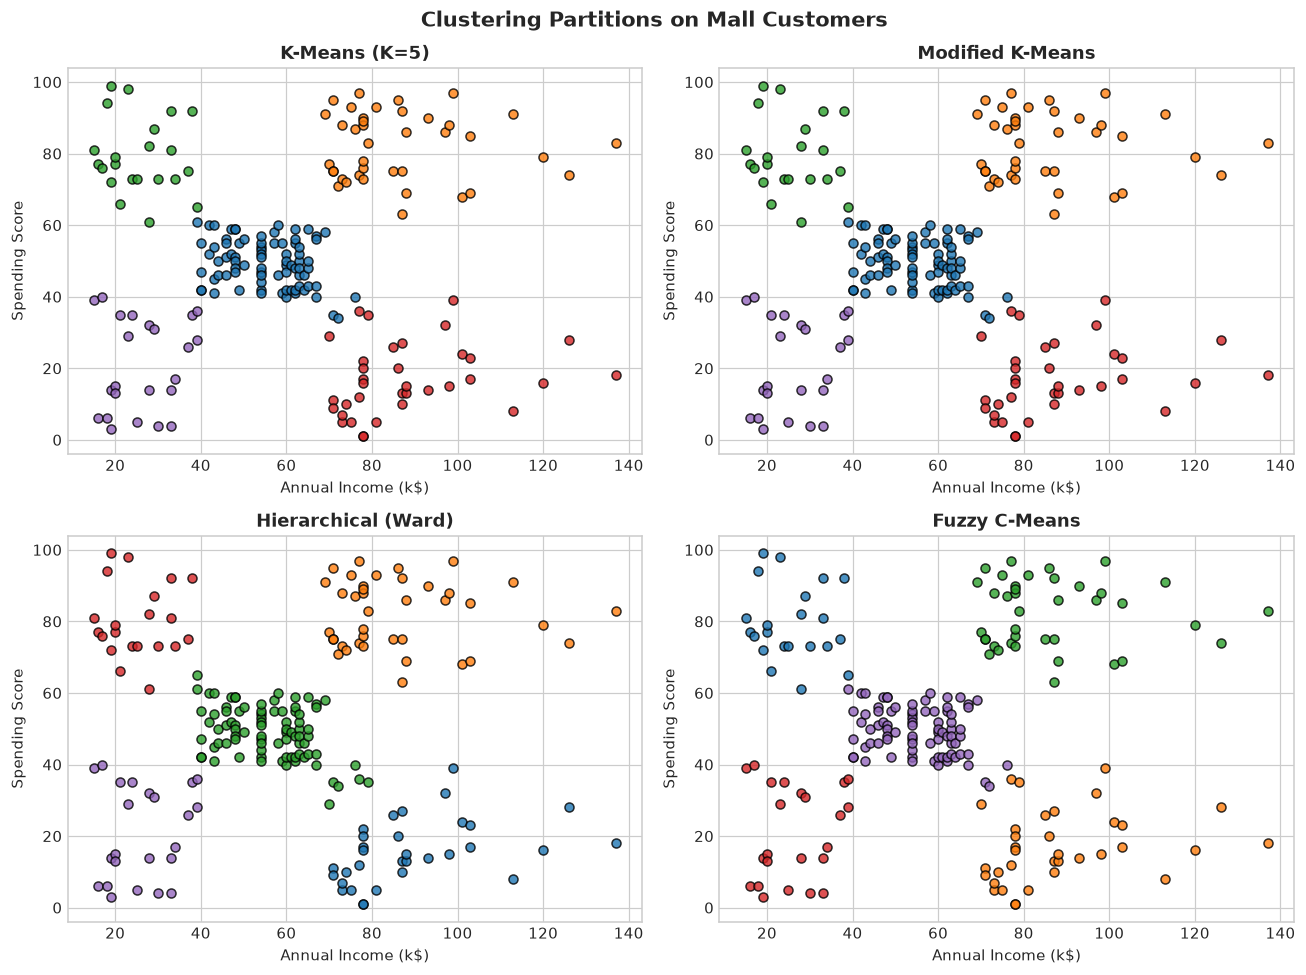
\includegraphics[width=0.95\textwidth]{figures/exp01_2x2_grid.png}
  \caption{Clustering partitions on the Mall Customers data: K-means, modified K-means
  (outlier flagging), hierarchical Ward and Fuzzy C-means.}
  \label{fig:exp01-grid}
\end{figure}

\section{Viva / Discussion Questions}
\begin{description}
  \item[How is Fuzzy C-means different from K-means?] It assigns membership degrees instead
  of hard labels, so each point belongs to all clusters with weights that sum to 1; K-means
  is the limiting hard case.
  \item[What does $m$ control?] The fuzziness exponent: larger $m$ spreads membership across
  clusters (softer, lower FPC), while $m \to 1$ gives crisp K-means-like assignments.
  \item[What does a membership vector represent?] The degree to which one observation
  belongs to each cluster; near-uniform values indicate an ambiguous point on a boundary.
\end{description}

\section{Complete Code Listing}
% ===========================================================================
% exp04_fuzzy_cmeans.tex - complete code listings for Experiment 4
% Source: notebooks/01_clustering_algorithms.ipynb (executed)
% Repository: https://github.com/Atik203/ML-Algorithms
% ===========================================================================

\begin{codebox}[title={Core numerical and plotting libraries}]
# ---- Core numerical and plotting libraries ----
import os
import numpy as np
import pandas as pd
import matplotlib.pyplot as plt
import seaborn as sns


# ---- Scikit-Learn clustering models ----
from sklearn.cluster import KMeans, AgglomerativeClustering
# ---- Feature scaling + unsupervised evaluation metrics ----
from sklearn.preprocessing import StandardScaler
from sklearn.metrics import silhouette_score, davies_bouldin_score, calinski_harabasz_score
# ---- SciPy hierarchical clustering utilities (linkage + dendrogram) ----
from scipy.cluster.hierarchy import dendrogram, linkage

# Styling setup (consistent look across all notebooks)
plt.style.use('seaborn-v0_8-whitegrid' if 'seaborn-v0_8-whitegrid' in plt.style.available else 'default')
plt.rcParams['font.sans-serif'] = 'DejaVu Sans'
plt.rcParams['figure.figsize'] = (10, 6)
plt.rcParams['figure.dpi'] = 110

# Fix the random seed so every run reproduces the same results
np.random.seed(42)
print("Libraries successfully imported!")
\end{codebox}

\begin{codebox}[title={Load the Mall Customers dataset}]
# ---- Load the Mall Customers dataset ----
df_mall = pd.read_csv('../data/mall_customers.csv')
print("Dataset Shape:", df_mall.shape)
print(df_mall.head(3))

# ---- Feature selection: two features so the clusters can be shown in 2D ----
X_mall = df_mall[['Annual Income (k$)', 'Spending Score (1-100)']].values

# ---- Standardize (mean = 0, std = 1): distance-based algorithms are scale-sensitive ----
scaler = StandardScaler()
X_mall_scaled = scaler.fit_transform(X_mall)
\end{codebox}

\begin{codebox}[title={Fuzzy C-Means class (from scratch)}]
class FuzzyCMeans:
    """
    Fuzzy C-Means (FCM) clustering - implemented from scratch with NumPy.

    Each sample belongs to every cluster with a membership degree u_ik in [0, 1],
    and the memberships over the K clusters sum to 1 per sample.

    Parameters
    ----------
    n_clusters   : number of fuzzy clusters K
    m            : fuzzifier exponent (m > 1; larger m => fuzzier memberships)
    max_iter     : maximum number of alternating-optimization iterations
    tol          : convergence tolerance on the maximum membership change
    random_state : seed for reproducible random initialization
    """

    def __init__(self, n_clusters=5, m=2.0, max_iter=150, tol=1e-5, random_state=42):
        self.n_clusters = n_clusters
        self.m = m
        self.max_iter = max_iter
        self.tol = tol
        self.random_state = random_state

    def fit(self, X):
        rng = np.random.RandomState(self.random_state)
        n_samples = X.shape[0]

        # Step 1: initialize the membership matrix U randomly and normalize every row to sum to 1
        U = rng.rand(n_samples, self.n_clusters)
        U = U / U.sum(axis=1, keepdims=True)

        # Step 2: alternate between centroid and membership updates until convergence
        for iteration in range(self.max_iter):
            U_old = U.copy()

            # 2a: centroid update - membership-weighted mean of the data
            Um = U ** self.m                                        # u_ik^m
            centers = np.dot(Um.T, X) / Um.sum(axis=0)[:, np.newaxis]

            # 2b: compute the (n_samples x n_clusters) distance matrix to every centroid
            dist = np.linalg.norm(X[:, np.newaxis, :] - centers[np.newaxis, :, :], axis=2)
            dist = np.fmax(dist, 1e-10)  # avoid division by zero

            # 2c: membership update - closer points receive higher membership
            #     u_ik = 1 / sum_j (d_ik / d_ij)^(2/(m-1))
            inv_dist = 1.0 / dist
            power = 2.0 / (self.m - 1.0)
            inv_dist_p = inv_dist ** power
            U = inv_dist_p / inv_dist_p.sum(axis=1, keepdims=True)

            # 2d: stop when memberships stop changing (convergence)
            if np.max(np.abs(U - U_old)) < self.tol:
                break

        # Store results: final centroids, full membership matrix, and hard labels
        self.cluster_centers_ = centers
        self.u_ = U
        self.labels_ = np.argmax(U, axis=1)  # hard assignment = cluster with maximum membership
        return self


# Fit FCM with the same K as the other algorithms (m = 2 is the standard fuzzifier)
fcm = FuzzyCMeans(n_clusters=optimal_k, m=2.0, random_state=42)
fcm.fit(X_mall_scaled)
fcm_labels = fcm.labels_
fcm_centers = scaler.inverse_transform(fcm.cluster_centers_)

# ---- Evaluation of the hard partition induced by the fuzzy memberships ----
print(f"FCM Silhouette Score: {silhouette_score(X_mall_scaled, fcm_labels):.4f}")
print(f"FCM Davies-Bouldin Index: {davies_bouldin_score(X_mall_scaled, fcm_labels):.4f}")
fpc = np.mean(np.sum(fcm.u_ ** 2, axis=1))   # fuzzy partition coefficient (1/K fuzzy ... 1 hard)
print(f"FCM Fuzzy Partition Coefficient (FPC): {fpc:.4f}")
\end{codebox}

